\chapter{Критерии идентификации}

\section{Свойства и параметры критериев идентификации}

Особенность динамики хаотических систем не позволяет
определить цель идентификации как задачу минимизации
какой-либо меры $\mu(x_o(t),x_i(t))$ в пространстве выходных
сигналов~[].

\Cmt{TODO: обоснование и картинки}

На рис.~\ref{atu:f:lor_diff_x0} приведён пример, показвающий
различие траекторий для системы Лоренца \Cmt{ref}
при малом возмущении значений начальных условий.

\begin{figure}[h!]
  \centerline{
    \includegraphics[width=0.49\textwidth]{p/lor_diff-p_xx_x0.png}
    \hfill
    \includegraphics[width=0.49\textwidth]{p/lor_diff-p_dx_x0.png}
  }
  \caption{Различине в поведение системы Лоренца при малом возмущении начальных условий}
  \label{atu:f:lor_diff_x0}
\end{figure}


На рис.~\ref{atu:f:lor_diff_sigma} приведён пример, показвающий
различие траекторий для системы Лоренца
при малом возмущении значений параметра $\sigma$.

\begin{figure}[h!]
  \centerline{
    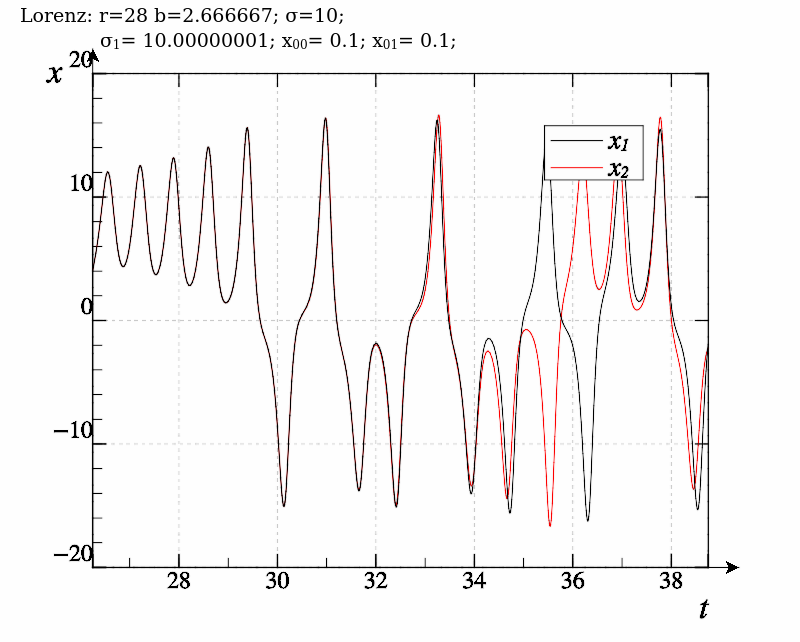
\includegraphics[width=0.49\textwidth]{p/lor_diff-p_xx_sigma.png}
    \hfill
    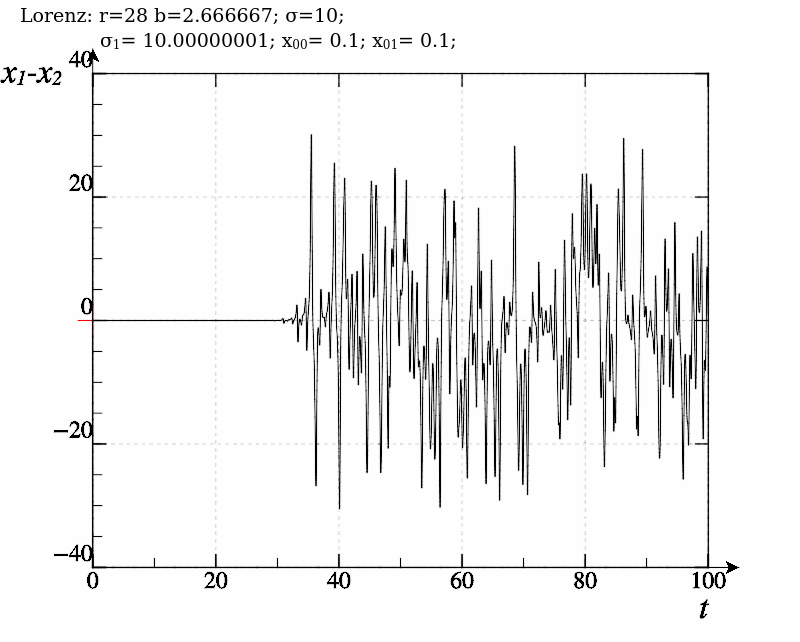
\includegraphics[width=0.49\textwidth]{p/lor_diff-p_dx_sigma.png}
  }
  \caption{Различине в поведение системы Лоренца при малом возмущении параметра $\sigma$}
  \label{atu:f:lor_diff_sigma}
\end{figure}


Для целей идентификации необходимо существование
заданного скалярного критерия $q(x(t))$, близость величин
которых для объекта и модели (в смысле какой-либо меры)
и позволяет говорить о достижении цели идентификации.

Физическая измеримость.

Следствием невозможности непосредственного использования выходных
сигналов объекта и моделей в качестве критерия идентификации, а также
требование физической измеримости критерия является
тот факт, что для получения оценки критерия, как правило,
требуется значительное время.

Законы сохранения в физике.

Представления величин, связанных с энергией.

Voltage, elastic -- $x^2$.

Potential in uniform field -- $x$ 

Chemical kinetic -- $\max(x)$.

Electro-magnetic -- $x\cdot y$.



Отношение к интересующим аспектам динамики объекта.

Монотонность -- как следствие одноэкстремальность?


Зависимость (обозначение?) от времени оценивания.
Методы измерения.






\section{Отличие задачи идентификации от задач решения нелинейного уравнения и поиска экстремума}

\Cmt{Перенести куда-то}

На первый взгляд, при заданном критерии идентификации, задача идентификации
сводится к классической задаче решения нелинейного уравнения: надо найти такие значения
параметров $p$, при которых критерий модели (или какой-либо из моделей)
$q_m$ принимает значение, наиболее близкое к значению критерия объекта $q_o$:
\[
  \mu( q_o, q_m(p) ) \to \min.
\]
Или же при использовании функции качества идентификации $F(q_o, q_m )$ задача
эквивалентна классической задаче поиска экстремума:
\[
  F( q_o, q_m(p) ) \to \max.
\]
На самом деле, существуют определённые аспекты, которые делают такое
сведение практически невозможным.

Прежде всего, в задаче в обеих исходных задачах
предполагается, что наблюдаемая система статична:
значение критерия не зависит от времени, и проведя измерение
в точке один раз, можно к нему не возвращаться.
Напротив, идентификация динамической системы предполагает,
что значение критерия, даже после какого-либо усреднения на конечном
интервале времени, есть величина динамическая, причём динамика определяется
не только параметрами системы, но и свойствами самой системы измерения,
а также процессом взаимодействия системы измерения с моделями. При этом
возможны весьма нетривиальные явления, такие как параметрический
резонанс, распространение параметрических волн на множестве моделей и т.д.

Также существенную роль могут играть как шумы измерения, так и побочные
эффекты от процесса фильтрации шумов.
Применение практически любого фильтра приводит к запаздыванию
в процессе измерения, и игнорирование этих явлений может привести
как к нарушению устойчивости поиска, так и получению совершенно
неадекватных результатов при наличии устойчивости.

В исходных задачах предполагается, что не только
значение функции известно точно в каждой точке, но также известны все производные
(по крайней мере, необходимые для работы метода).
В реальные задачах идентификации производные непосредственно
не доступны для измерения, а их оценка требует применения специальных
методов. При этом процесс оценивания производных, как правило,
более чувствителен к шумам измерения, чем собственно измерение.


\Cmt{ TODO: Требование конечности производных в условиях дискретного представления сигнала.}

Все эти явления делают задачу идентификации более сложной, чем
исходные задачи, чем и обусловлено
существование широкого спектра методов идентификации. Тем не менее,
некоторые алгоритмы, применимые при поиска экстремума, могут быть
полезны при синтезе системы идентификации.

Свёртка с чем-то.

Как уже было отмечено, для успешности процесса идентификации требуется
построение различных интегральных критериев, зависящих,
хотя бы в первом приближении
от величины идентифицируемого параметра. Конкретный вид определяется самим идентифицируемым
объектом. При этом, довольно часто (но не всегда) в качестве основы для такого критерия выступает
некая энергетическая зависимость. С учётом усреднения на требуемом интервале,
один из простых видов критерия может быть задан как
%
\begin{equation}
\od{q_{x^2}}{t}
=
\frac{1}{\tau_q} \left( x^2(t) - q_{x^2}(t) \right)
,
\label{atu:eq:qlin}
\end{equation}
%
%\noindent
где $\tau_q$ -- характерное время оценивания, $x(t)$ -- выбранная переменная состояния системы.

Скользящее среднее:
$q_{ma}$??

Чернавскиий~\cite{chernavskii_syn_info}.

\section{Выводы по разделу \thechapter}

Выводы.

